\subsection{CNN}
\label{CNN-label}

Our Convolutional Neural Network image classifier was our best model by a narrow margin. We do not include a block diagram of the key algorithmic components as the image processing was quite simple and limited to augmentation consisting of blurring and rotation.  

Our network was based on lab code \cite{INM460-lab-wk8}. Some alternative network architectures were tried, with added layers, different learning rates and epochs. We could not improve on the network given in class and in the end used it without modification, that is, two stacks of convolutional, batch normalization, rectified linear unit and max pooling layers, followed by the same stack excluding max pooling layer, followed by a fully connected, softmax and classification layer. For grayscale images, we changed the dimensions of the image input layer, to account for the single colour channel.

We varied training epochs from 2 to 32 and found that 4 was an adequate number (Figure \ref{fig:cnn_training_progress} - dark continuous curve: training accuracy smoothed, light continuous curve: training accuracy, dashed lines: validation accuracy), as the network had usually converged by then to a stable accuracy value that was unlikely to change with the addition of more epochs.

\begin{figure}[h]
 \centering 
 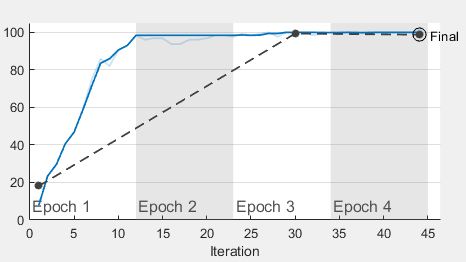
\includegraphics[width=\columnwidth]{images/cnn-training-progress.png}
 \caption{CNN training progress showing conversion after three epochs, for 200 samples per label, 128x128 pixel RGB images}
 \label{fig:cnn_training_progress}
\end{figure}

We used function \textbf{fnTrainCNN} to train our networks. This returned the trained network and accuracy as output parameters, used to build Table \ref{table:cnn_stats} in section \ref{Appendix}. The outputs showed that our networks worked better with smaller images, consistently generating higher accuracies for grayscale image sizes of 70x70 pixels. Overall, networks trained using grayscale images performed slightly better than the RGB counterparts on individual images, which suggests variability such as introduced by differing light conditions might have been attenuated in grayscale images. 

We tried using grayscale images as a single channel input to our convolutional neural network as they trained faster than 3 channel RGB images. We tested our grayscale image network on one group image (class2.jpg), using our \textbf{RecogniseFace} function. One in twenty images was classified correctly. Compared to 4 in 20 using our best RGB model. The reason for the lower performance of grayscale images on group images may be related to further processing being required in group images, as performance on individual images was better for grayscale than RGB images. We discuss this in section \ref{Discussion-marker}.

Based on ad hoc testing and grid search results, 70x70 pixel RGB images were chosen to train the coursework CNN models. Figure \ref{fig:cnn_correct_incorrect} shows a detail of image generated by our \textbf{RecogniseFace} function with one correct and one incorrect classification
\begin{figure}[ht]
 \centering 
 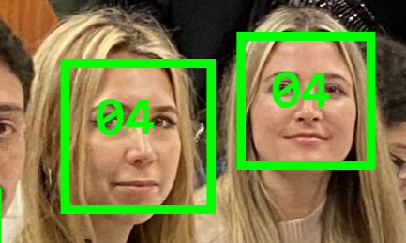
\includegraphics[width=\columnwidth]{images/correct-incorrect.png}
 \caption{Correct (left) and incorrect (right) classification labels from CNN trained with 70x70 pixel RGB images}
 \label{fig:cnn_correct_incorrect}
\end{figure}

